%%%%%%%%% PROPOSAL -- 15 pages (including Prior NSF Support)

\section{Project Description}
\subsection{Introduction}

164 years have passed since Darwin admitted that altruism may be the one flaw in his theory of evolution. Cooperation is the donation of an aspect of an organism's survival, growth, or ability to reproduce in order to help another organism, and altruism is a type of cooperation in which the cooperative behavior does not result in the donor receiving a direct fitness benefit in return within its lifetime \cite{west_social_2007}. There are many types of cooperative behaviors that differ in the component of fitness being donates, which can be thought of as their ecological currency. These different types of cooperative behaviors may by the aspect of fitness which is donated or exchanged; three broad categories are fecundity, resources, or survival \cite{van_dyken_origins_2012}.  One type of cooperative behavior can, through its ecological currency, alter the environment and the altruistic species' social structure in a way that feeds back on the evolution of other cooperative traits with distinct ecological currencies; this process is called reciprocal niche construction \cite{odling-smee_niche_1996}. For example, resource altruism has been hypothesized to decrease local competition between group members, making them more likely to help each other breed even if relatedness between group members is low \cite{van_dyken_origins_2012_II} 

However, exceedingly few theoretical or empirical studies have investigated the effects of niche construction of cooperative traits, nor the reciprocal niche construction that may allow high levels of cooperation between kin or even non-kin to evolve. This gap is not only a disservice to the field of evolutionary biologists studying the evolution of cooperation, but also to ecology and conservation. Many species that are considered to structure their local communities, such as sea otters  \cite{estes_killer_1998, estes_sea_2016}, orcas \cite{estes_killer_1998, valls_keystone_2015}, and wolves \cite{c_eisenberg_wolfs_2013} are also extremely social, and of the few studies examining the topic, their social behavior can alter and be altered by their interactions with other species \cite{jordaan_effect_2023, imbert_why_2016, foster_social_2012}. Very little modeling has studied the influence of the evolution of social behavior on the population dynamics of predators and prey. Previous work has examined how the evolution of social learning and cooperation influences prey choice and prey population dynamics in a one-predator, two-prey model where the predator population was held constant \cite{borofsky_static_2022, borofsky_success-biased_2022, borofsky_cultural_2024}, and one model has examined the influence of social learning by predators in a one predator, one prey model where both poplations changed \cite{kikuchi_social_2023}. Previous work on cooperation in predator-prey models have modeled cooperation as an allee effect, assuming the capture rate of prey is a function of predator density rather than group size \cite{berec_impacts_2010, teixeira_alves_hunting_2017}, even though studies of social species have largely been unable to observe population-level allee effects \cite{lerch_why_2018}. The only paper with a predator functional response that incorporated sharing and  was a function of predator group size rather than predator population size, assumed that predator groups do not improve capture probability of prey \cite{fryxell_group_2007}.

Additionally, group structured-populations remain a challenge to ecological and evolutionary models of social behavior. Group-selection models have sought to examine how cooperative traits may spread by increasing the competitive advantage, and hence relative fitness, of groups with more cooperators, but these models generally do not both allow for group formation and for for individuals to leave or join groups if it will increase their own fitness \cite{traulsen_evolution_2006, simon_towards_2013}. However, many social predators are increasingly recognized to live in groups with flexible group membership \cite{smith_social_2008, } \red{(also unpublished observations from Adrian Treves of solves switching groups)}

Here, the P.I. focuses on cooperative hunting and reproductive skew resulting from fecundity altruism. Cooperative hunting describes predators hunting a prey item as a group and sharing the resulting kill, and may be most advantageous if it allows predators to expand their niche by hunting prey they could not catch otherwise. Reproductive skew is the uneven distribution of resources among organisms. It can arise randomly \cite{steiner_neutral_2012, tuljapurkar_skewed_2020}, but in many types of cooperative organisms, including ants \cite{holldobler1990ants} and hyenas \cite{holekamp_rank_1996}, socially-enforced hierarchies generate extreme reproductive skew. Here, the P.I. aims to (1) understand how resource-based cooperation, and specifically cooperative hunting, influences and is influenced by prey abundance, (2) examine the feedback between cooperative hunting and the evolution of reproductive skew caused by fecundity altruism. 

The P.I. proposes to conduct three projects:
\begin{enumerate}
\item The interaction of group formation dynamics and population dynamics
\item The evolution of reproductive skew with a population structured into groups that can hunt cooperatively or solitarily.
\item meta-analysis of cooperative hunting behavior, group dynamics, and reproductive cooperation across carnivora
\end{enumerate}

\subsection{Project 1: Predator Group Formation and Prey Dynamics}
% From the NSF Grants Proposal Guide:
% "The Project Description should provide a clear statement of the work 
% to be undertaken and must include: objectives for the period of the proposed 
% work and expected significance; relation to longer-term goals of the PI's 
% project; and relation to the present state of knowledge in the field, 
% to work in progress by the PI under other support and to work in progress 
% elsewhere."
The predator population, with population size $p$, hunts two types of prey: big prey, with population size $M_1$, and small prey, with population size $M_2$. Big prey and small prey are also referred to as prey types 1 and 2, respectively. Predators are split into hunting groups that are of size $x \in 1, 2, \cdots, p$. Let $f(x,t)$ be the number of groups of size $x$, which for brefity is also written as $f(x)$, so that the portion of predators in a group of size $x$ is $\bar{f}(x) = x f(x)/p$. The population dynamics of predators and prey are 
\begin{subequations} \label{general_model}
\begin{align}
\frac{dp}{dt} &=  \sum_{x=1}^{\xm} f(x) \lrb{b_1 Y_1(x,M_1,M_2) + b_2 Y_2(x,M_1,M_2)} - p \delta \\
\frac{dM_1}{dt} &= g_1 M_1 \lrp{1 - \frac{M_1}{k_1}}  -  \sum_{x=1}^{\xm} f(x) Y_1(x,M_1,M_2) \\
\frac{dM_2}{dt} &= g_1 M_1 \lrp{1 - \frac{M_1}{k_1}}  -  \sum_{x=1}^{\xm} f(x) Y_2(x,M_1,M_2)
\end{align}
\end{subequations}
where the parameters are defined in Table \ref{originalparameters} and $Y_i(x,M_1,M_2)$ is the functional response on prey $i$. The functional responses are defined as the rate of prey caught per hunting \textit{entity}, i.e. a solitary predator or predator group, so the fitness from hunting in a group is shared across the group WHICH IS NOT PRESENT IN OTHER PRED-PREY MODELS WITH COOPERATIVE HUNTING. The functional response of a hunting group of size $x$ is a type II functional response (CITE HAMILTON?), namely
\begin{equation} \label{fun_response}
Y_i(M_1, M_2, x) = \frac{a_i \alpha_i(x) M_i}{1 + \sum_{j=1,2} a_j \alpha_j(x) h_j M_j}, \qquad \alpha_i(x) = \frac{1}{1 + e^{-\theta_i(x - s_i)}}
\end{equation}	
for $i = 1,2$. The parameters are defined in Table \ref{originalparameters}. Importantly, the predator group size influences the capture probability $\alpha_i(x)$, which is the probability a predator captures prey $i$ upon encounter (Fig. \ref{fig_capture_rates}). However, the combination of parameter $\theta_i, s_i$ are not very intuitive for understanding how the capture probability responds to group size, especially since increasing $\theta_i, s_i$ also changes the capture probability of solitary predators. For $\alpha_{i}(1)$ the capture probability of prey $i$ by solitary predators, $\theta_i = - \frac{\ln\lrp{ \frac{1}{\alpha_i(1)} -1 }}{1 - s_i}$ is substituted into eq. \ref{fun_response}.

\begin{wrapfigure}{l}{0.5\textwidth}
\begin{center}
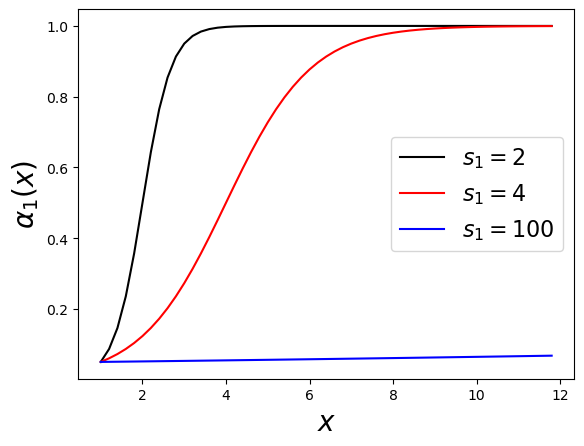
\includegraphics[width=.4\textwidth, trim={0 0.3cm 0 0},clip]{Figures/capturerate_bigprey.png}
\end{center}
\caption{Capture probabilities of big prey if $\alpha_1(1)= 0.05$ for big prey and $\alpha_2(1) = 0.95$ for small prey, for different critical group sizes ($s_1$)}
\label{fig_capture_rates}
\end{wrapfigure}

\begin{table}[h]
\caption{List of parameters used in Project 1}
\begin{center}
\begin{tabular}{|c|p{5in}|}
\hline
\textbf{Parameter} & \textbf{Definition}  \\
\hline
$b_i$ & Conversion of prey $i$ caught to predators; $b_1 > 0 $ and $0 < b_2 < b_1$ \\
\hline
$\delta$ & Death rate of predators, i.e. the probability a predator dies per unit ecological time; $\delta > 0$\\
\hline
$\tau_x$ & The time constant for the dynamics of group size \\
\hline
$\theta_1$ & Facilitation by cooperation of predators hunting big prey; $\theta_1 \geq 0$ \\
\hline
$\theta_2$ & Facilitation by cooperation of predators hunting small prey; $\theta_2 \leq 0$ \\
\hline
$s_i$ & Critical group size for predators hunting prey type $i$, $s_i > 1$. \\
\hline
$h_i$ & Handling time of prey type $i$\\
\hline
$a_i$ & Attack rate on prey type $i$ \\
\hline
%$\gamma$ & Portion of even share of food donated by subordinates \\
%\hline
%$r$ & Average relatedness between the dominant and subordinates \\
%\hline
\end{tabular}
\end{center}
\label{originalparameters}
\end{table}%
Predators may leave and join groups multiple times within their lifespan. The time constant for group dynamics is $\tau_x$. While time for the population dynamics processes in system eqs. \ref{general_model} is on the order of years or seasons, time for group dynamics may be on the order of days, so $\tau_x << 1$. Thus the group size distribution changes from the following processes: (1) solitary individuals join group of size $x$ at rate $\psi(x)$, (2) individuals leave groups of size $x$ at rate $\phi(x)$, (3) Individuals die at rate $\delta \tau_x$, the death rate relative to the time scale of group dynamics, and (4) individuals are born at a rate that is the yield from hunting, adjusted for the group formation time scale, i.e. $\tau_x f(x) \pi(x)$ , where $\pi(x) = b_1 Y_1(x) + b_2Y_2(x)$ is the yield from hunting. After birth, offspring initially are in their natal group unless they are born in a group of the maximum group size, in which case they become solitary. The master equations for the number of solitary individuals, the number of groups of size 2, and number of groups of size $x \geq 2$, are, respectively,
\begin{multline} \label{df_of_1}
\tau_x \pdv{f(1)}{t} =\ + \underbracetwo{2 \cdot f(2) \phi(2)}{groups of 2}{split to two solitaries} \ +  \underbracetwo{\sum_{x=3}^{\xm} f(x) \phi(x)}{individuals leave}{larger groups}\ 
 -\  \underbracetwo{ f(1) \sum_{x=2}^{\xm} \psi(x-1)}{solitaries join}{groups}  \\+  \underbracetwo{\tau_x \lrc{ f(x_m) \pi (x_m ) - f(1) \pi(1) + \delta \lrb{2f(2) - f(1)}}}{ births and deaths}{},
\end{multline}
\begin{multline} \label{df_dt_2}
\tau_x \pdv{f(2)}{t} = \ -\  \underbracetwo{f(2) \phi(2)}{an individual}{leaves} 
\ - \ \underbracetwo{f(2) \psi(2) }{growing to}{larger group} \ +\  \frac{1}{2} \underbracetwo{f(1) \psi(1)}{solitaries}{forming dyads}\ +\ \underbracetwo{f(3)\phi(3)}{a member leaves }{a larger group}\\
+ \underbracetwo{ \tau_x \lrc{f(1) \pi(1) - f(2) \pi(2) + \delta \lrb{ 3 f(3) - 2 f(2)  } } }{births and deaths}{},
\end{multline}
and for $x > 2$,
\begin{multline} \label{df_dt}
\tau_x \pdv{f(x)}{t} = -\underbracetwo{  f(x) \phi(x) }{an individual}{leaves} \ - \ \underbracetwo{f(x) \psi(x) }{growing to}{larger group} \ +\ \underbracetwo{f(x-1)\psi(x-1)}{smaller group}{grows to size $x$} + \underbracetwo{f(x+1)\phi(x+1)}{a member leaves}{a larger group}\\
+ \tau_x \lrc{ f(x-1)\pi(x-1) - f(x) \pi(x) + \delta \lrb{(x+1)f(x+1) - xf(x)} }.
\end{multline}

Let $S(x,y)$ be the best response function modeling the probability a decision-maker will transition from a group of size $y$ to a group of size $x$, for $x,y \geq 1$, $y \leq \xm$, and $x \leq \xm - 1$. If predators can freely leave and join groups, then that decision-maker is the predator that is deciding whether to leave or join a group. If groups decide whether to admit or eject members, the decision-maker could be either any subordinate individual in a group or the dominant individual. This function is sigmoidal in shape, growing closer to $1$ as the per capita fitness difference $\frac{1}{x} \pi(x) - \frac{1}{y}\pi(y)$ increases. We model this choice using Tullock's contest success function \cite{tullock_efficient_1980}, i.e.,
\begin{equation} \label{best_response_function}
S(x,y) = \frac{\lrp{\frac{1}{x}\pi(x)}^d}{\lrp{\frac{1}{x} \pi(x)}^d + \lrp{\frac{1}{y}\pi(y)}^d}
\end{equation}
for $d$ a positive scaling constant that determines the shape of $S(x,y)$. If individuals can freely join or leave groups, the rate at which individuals join a group of size $x$ is
\begin{equation}
\psi(x) = 
\begin{cases}
\lrb{f(1) - 1} S(2,1) & \text{if } x = 1 \text{ and } \red{f(x) \geq 1}\\
f(1) S(x+1,1)  & \text{if } 1 < x \leq \xm - 1 \\
0 & \text{otherwise},
\end{cases}
\end{equation}
\red{If $F(1)<1,$ what should I do???? Should it just be $F(1)^2$?}
and the rate at which they leave a group of size $x$ will be $\phi(x) = xS(1,x)$ for $x \leq \xm$.  

This model can be partially non-dimensionalized, scaling the population sizes of big prey and small prey by their carrying capacities, so $N_1 = M_1/k_1$ for big prey and $N_2 = M_2/k_2$ for small prey. The population time-scale constant is $\hat{t} = g_1 + g_2 + \delta$, with non-dimensionalized time $T = t \hat{t}$ and the group dynamics time constant $T_x = \hat{t} \tau_x$. For $\xi = \hat{t}/(a_1 + a_2)$ the ratio of the predation-independent growth rates to the attack rates, the predator population is scaled to $P = p/\xi$ and the number of groups of size $x$ is $F(x) = f(x) /\xi$. The new parameters are $\eta_i = g_i/\hat{t}$, $A_1 = a_1/(a_1 + 1_2)$, $\beta_i = a_i b_i k_i/\hat{t}$, and $H_i = a_i h_i k_i$. It is not useful to non-dimensionalize group size, $x$.

\subsubsection{Plan for Analysis and Preliminary results}
The P.I.'s intend to compare the model described in eqs. \ref{general_model}a - c and eqs. \ref{df_of_1} - \ref{df_dt} to a model in which all predators are in groups of size $x^*$, described by eqs. \ref{general_model}a - c with $f(x) = p/x$ for $x = x^*$ and 0 otherwise. Initial results indicate that whereas restrincting group sizes to stay at a constant $x^*$ can lead to one prey type going extinct, allowing fission-fusion dynamics of group sizes results in both prey types and predators coexisting. The P.I.'s will test whether increased availability of prey selects for more cooperation by examining whether increasing growth rates of big prey expected group size to which a randomly selected predator belongs, $\bar{x} = \sum x \bar{f}(x)$,  by calculating $\pdv{\bar{x}}{N1}$ at the equilibrium, and by testing whether an increase in the growth rate of big prey, $g_1$, leads to an increase in $\bar{x}$. Furthermore, they will examine the range of parameters for which extinction of either prey type is locally stable using linear stability analysis. Finally, the authors will examine the presence or absence of apparent competition, as defined in \cite{holt_predation_1977}, between prey types, and whether apparent competition depends on group dynamics.



\subsection{Project 2: The Evolution of Reproductive Skew across Dynamic Groups}

DO I NEED THE SMALL PREY VS BIG PREY HERE, OR IS IT ENOUGH TO JUST SAY THEY GET A BIG YIELD IN A GROUP BUT IT HAS TO BE SHARED, THEY GET A SMALL YIELD ALONE BUT IT'S ALL THEIRS.
\subsubsection{Cooperative Hunting}
Predators can hunt large prey, which has benefit $b_1$ before sharing, or hunt small prey which has benefit $b_2$ before sharing. There are no population dynamics of big prey and small prey, but predator grouping increases the capture probability of big prey. The rate at which predator groups catch prey is similar to eq. \ref{fun_response} but $M_1, M_2 = 1$. Since there should be a trade-off between the amount of effort spent on one prey on the amount of effort available on the other prey, there is handling time for prey, but since handling time is not the focus, it is set to $h_1 = h_2 = h$. Additionally, to increase tractibility the attack rates of both prey are the same and set at $a_1 = a_2 = 1$. Thus if all predators spend all their time foraging, then the group's yield (i.e. number of offspring) from hunting is
\begin{equation} \label{fun_response_2}
\pi(x) = \frac{b_1 \alpha_1(x) + b_2 \alpha_2(x)}{1 +  h \alpha_1(x) + h \alpha_2(x)} \qquad \text{for }
\alpha_i(x) = \frac{1}{1 + e^{-\theta_i(x - s_i)}}.
\end{equation}
\subsubsection{Reproductive Skew}
Reproductive skew will be represented in one of the following ways:
\begin{enumerate}
\item Public Goods Game: If the yield from prey is first split evenly, such that each individual in a group of size $x$ receives yield $\frac{1}{x} \pi(x)$, and subordinates sacrifices a portion $\gamma$ to the dominant, then the direct fitness of subordinates is $w_s(x) = \frac{\pi(x)}{x}(1-\gamma)$ and that of the the dominant is $u\frac{1}{x} \pi(x) \lrb{1 + \gamma(x-1)}$, where $u>1$ is a multiplication factor.
\item Division of Time Budgets: Predators split their time between foraging and reproducing, so by sacrificing a portion of their reproductive effort $\gamma$, subordinates also decrease their time reproducing by $\gamma$ and thus spend more time hunting. The dominant decreases its time hunting by $\gamma$ for each subordinate in the group. Thus as $\gamma$ increases, the expected number of hunters that are actively hunting at any given moment of time increases.
%\item Decreasing Sunk Costs: The amount of reproduction a predator can do with respect to how much food it receives is sigmoidal. Then if a group does not hunt a lot of food and shares it evenly, everyone reproduces very little, but if the dominant instead receives most of the food, their collective reproduction is much higher. THIS WOULD SELECT FOR REPRODUCTIVE SKEW IF THERE IS A LOT OF STOCHASTICITY
\end{enumerate}
%Let $w_s(x), w_d(x)$ be the direct fitnesses of a subordinate and a dominant, respectively. WHAT IF WE EXPLORE GROUP SELECTION THEORIES WITH NO RELATEDNESS? HOW ARE WE DEFINING THIS RELATEDNESS ANYWAYS? RELATEDNESS RELATIVE TO RELATEDNESS IN THE POPULATION? For $r_s$ the average relatedness between subordinates in a group and $r_d$ the average relatedness between subordinates and the dominant in a group, the inclusive fitness of subordinates and the dominant are
%$$
%W_s(x) = w_s(x)\lrb{ 1 + r_s (x-2) } + r_d w_d(x) \qquad \text{and} \qquad W_d(x) = w_d + r_d (x-1) w_s(x), 
%$$
%respectively. 

\subsubsection{Group Fission and Fusion}
As in project 1, $f(x)$ is the number of groups of size $x$. Here, offspring initial stay in their native group. One individual in a group is a dominant and the rest are subordinates, but every group member has a uniform probability $1/x$ of being a dominant. As in Project 1, $\psi(x), \phi(x)$ are the rates at which predators join and leave a group, respectively. If predators are able to freely leave and join groups, then when a predator is deciding to join or leave a group, it compares its solitary fitness to the expected fitness in the group. If groups control whether predators can stay or join, then a predator leaves a group if the group's fitness increases by decreasing group size. A predator joins a group if its own fitness increases by joining the group and if the group's fitness increases by augmenting group size. Since this model does not focus on population dynamics, population size is held constant by balancing the birth rate of the population with the death rate. For $W(x)$ the total birth rate of a group of size $x$, then because $\sum_x f(x) W(x)$ is the overall birth rate of the population, the per-capita death rate is $\delta = \frac{1}{p} \sum_x f(x) \bar{w}(x)$ for $p = \sum_x x f(x)$ the constant population size.


\subsection{Project 3: The Presence of Cooperative Hunting, Cooperative Breeding, and Group Formation across Carnivora}
This project explores trends in the social behavior and ecology of Carnivora with the aim of comparing the ecology and social behaviors of predators that hunt alone, those that hunt in groups but do not cooperate, and those that both hunt in groups and cooperate. Previous work exploring the diversity of social hunting strategies has focused on exploring types of hunting behaviors among predators that are social, rather than doing a thorough comparison of species that are solitary and social \cite{hansen_mechanisms_2023, lang_multidimensional_2017, bailey_group_2013}. In particular, the P.I.'s intend to investigate whether predators that hunt cooperatively also breed cooperatively. The P.I.'s focus on Carnivora because it is a relatively small order (only around 270 species) made up of predators that contains well known examples of cooperative hunters, solitary hunters, and cooperative breeders, including some species that use a mix of solitary hunting and cooperative hunting.

The P.I. will mentor a high school student to collect the following information, where available, on species of carnivora:
\begin{enumerate}
\item \textbf{Group Hunting Characteristics} - Whether the predator hunts in groups, the size of those groups, the degree of collaboration and sharing while hunting, and whether both sexes or just one sex hunts in groups.
\item \textbf{Cooperative Breeding} - Whether females raise young in groups (i.e., in the presence of adult conspecifics), the degree of reproductive skew in groups, whether some adults help rear the young of other adults, and the presence of infanticide in groups.
\item \textbf{Prey characteristics} - The types of prey hunted in groups and alone, the size of the prey relative to the predators, and the sociality of the prey.
\end{enumerate}


\section{Broader Impacts}
% as in the project summary, broader impacts must be called out separately 
% in the project description.  You may be able to give more specific
% examples, or discuss how you've previously achieved these impacts.
% It should be similar, but not identical, to the Broader Impacts statement
% in the project summary

\section{Results From Prior NSF Support}
% 5 pages or fewer of the 15 pages for entire description document.
% include results from NSF grants received in the past 5 years.
% if supported by more than one grant, choose the most relevant one
% for each grant, include: NSF award number, amount, dates of
% support, and publications resulting from this research.
% due to space limitations, it is often advisable to use citations rather
% than putting the titles of the publications in the body 
% of this section

% e.g.: "My prior grant, "Uses of Coffee in Mathematical Research" (DMS-0123456, 
% $100,000, 2005-2008), resulted in 3 papers [1],[2],[3], demonstrating..."

% if requesting postdoctoral research salary, a supplemental 1-page document
% called "Postdoc Mentoring Plan" will be required